%
% ball.tex
%
% (c) 2026 Jack Dumovich, Roman Meyer
%
\documentclass[tikz,border=0pt]{standalone}

\usepackage{amsmath}
\usepackage{graphicx}
\usetikzlibrary{arrows.meta}
\usepackage{newtxtext, newtxmath} % Sets document-wide Times New Roman
\definecolor{rot}{rgb}{1,0,0}
\definecolor{bg}{rgb}{0,0,0}

\begin{document}
	
	\begin{tikzpicture}
		\clip (0,0) rectangle (12,9.375);
		
		% -------------------------------------------------
		% Background image
		% -------------------------------------------------
		\node[
		anchor=south west,
		inner sep=0
		] at (0,0)
		{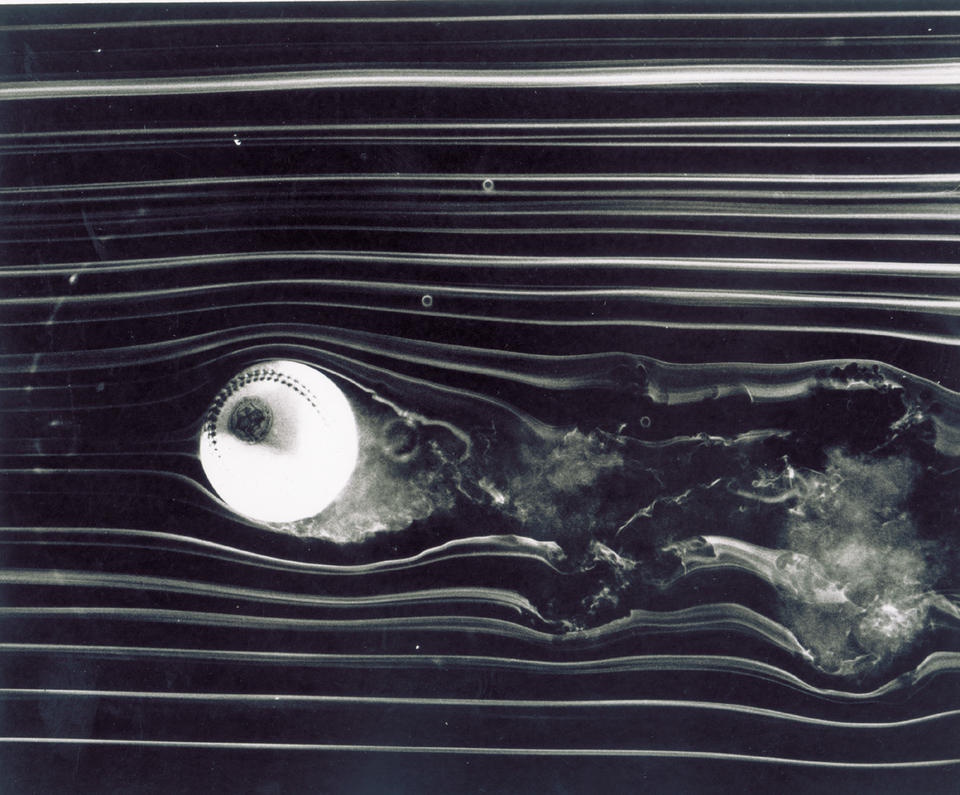
\includegraphics[width=12cm]{ball.jpg}};

		\fill[color=bg,opacity=0.6]
			(0.2,0) -- (2.7,0) -- ++(0,0.8) -- ++(-1.5,0)
			-- ++(0,1.7) -- (0.2,2.5) -- cycle;
		\fill[color=bg,opacity=0.6]
			(1,8.6) -- ++(1.8,0) -- ++(0,0.7) -- ++(-1.8,0) -- cycle;
		\fill[color=bg,opacity=0.6] (3.5,5.71) rectangle ++(0.75,0.7);

		
		% -------------------------------------------------
		% Red vectors
		% -------------------------------------------------
		
		% Freestream velocity V_infinity
		\draw[
		rot,
		line width=2.5pt,
		-{Latex[length=4.5mm,width=3mm]}
		]
		(1.20,8.82) -- (2.20,8.82);
		
		\node[
		rot,
		font=\Large
		] at (2.3,9.1)
		{$v_\infty$};
		
		
		% Vertical force F_y
		\draw[
		rot,
		line width=2.5pt,
		-{Latex[length=4.5mm,width=3mm]}
		]
		(3.45,4.28) -- (3.45,6.03);
		
		\node[
		rot,
		font=\Large
		] at (3.9,6.05)
		{$iF_y$};
		
		
		% -------------------------------------------------
		% Coordinate system
		% -------------------------------------------------
		
		% Origin
		\coordinate (O) at (0.71,0.43);
		
		% x-axis
		\draw[
		rot,
		line width=1.5pt,
		-{Latex[length=4.5mm,width=3mm]}
		]
		(O) -- (2.07,0.43);
		
		% y-axis
		\draw[
		rot,
		line width=1.5pt,
		-{Latex[length=4.5mm,width=3mm]}
		]
		(O) -- (0.71,1.83);
		
		% -------------------------------------------------
		% Coordinate labels
		% -------------------------------------------------
		
		% x label
		\node[
		rot,
		font=\Large
		] at (2.27,0.42)
		{$x$};
		
		% i and y in the same label
		\node[
		rot,
		font=\Large
		] at (0.78,2.08)
		{$i y$};
		
	\end{tikzpicture}
	
\end{document}
